\documentclass[11pt]{beamer}
\usetheme{Madrid}
\usepackage{amsmath,amssymb,amsfonts,graphicx}
\usepackage{multicol,multirow,booktabs}
\usepackage{tikz}
\usepackage{pgfplots}
\pgfplotsset{compat=1.17}
\usepackage{siunitx}
\sisetup{output-decimal-marker={.},separate-uncertainty=true}

% To fit long frames
\setbeamerfont{normal text}{size=\small}

\title{H2 Physics \\ Rotational Motion}
\author{R.F.H.}
\date{\today}

\begin{document}

\begin{frame}
\titlepage
\end{frame}

% Section 1: Getting Prepared
\section{Getting Prepared}

\begin{frame}[shrink=15]{Brain Dump}
\centering
\Large
\textit{What do you know about Rotational Motion?}
\vfill
\end{frame}

\begin{frame}[shrink=15]{Brain Dump (CONT'D)}
\centering
\Large
\textit{What do you know about Rotational Motion?}
\vfill
\begin{itemize}
    \item Torque $\tau = F \times r_{\perp}$ (moment of a force)
    \item Couple: two equal, opposite, parallel forces producing pure rotation
    \item Centre of gravity and moment of a force
    \item Equilibrium conditions: $\sum F = 0$, $\sum \tau = 0$
    \item Moment of inertia $I$ (rotational inertia)
    \item Angular acceleration $\alpha = \tau / I$
    \item Rotational kinetic energy $K_{\text{rot}} = \frac12 I \omega^2$
    \item Angular momentum $L = I \omega$
    \item Conservation of angular momentum
    \item Rolling motion (combination of translation and rotation)
\end{itemize}
\end{frame}

\begin{frame}{Math Checklist}
Before tackling Rotational Motion, ensure you are comfortable with:
\begin{columns}[T]
\column{0.5\textwidth}
\begin{itemize}
    \item Trigonometry ($\sin$, $\cos$, $\tan$)
    \item Vector cross products (direction of torque)
    \item Solving simultaneous equations
    \item Quadratic equations
    \item Differentiation and integration (for variable $\omega$)
\end{itemize}
\column{0.5\textwidth}
\begin{itemize}
    \item Radian measure
    \item Parallel axis theorem (if needed)
    \item Integration for moment of inertia (basic)
    \item Conservation laws
    \item Energy conservation with rotational terms
\end{itemize}
\end{columns}
\end{frame}

% Section 2: Concept Mastery
\section{Concept Mastery}

\begin{frame}{Building Intuition – Real-world Applications}
\begin{itemize}
    \item \alert{Seesaw}: balancing requires equal moments on both sides.
    \item \alert{Wrench}: longer handle gives more torque for the same force.
    \item \alert{Opening a door}: force applied farthest from hinges is most effective.
    \item \alert{Flywheel}: stores rotational energy to smooth engine pulses.
    \item \alert{Spinning figure skater}: pulls arms in to spin faster (conservation of angular momentum).
    \item \alert{Bicycle wheel}: gyroscopic effect helps with stability.
    \item \alert{Rolling ball}: combination of translation and rotation; energy split between $K_t$ and $K_r$.
\end{itemize}
\end{frame}

\begin{frame}{Formalization – Torque and Moment of a Force}
\begin{block}{Torque (Moment of a Force)}
\[\tau = F \times r_{\perp} = F r \sin\theta\]
where $r$ is the distance from pivot to point of force application, $\theta$ is angle between force and lever arm.
\end{block}
\begin{block}{Couple}
Two equal and opposite forces, not collinear, produce a torque $\tau = F \times d$ (where $d$ is perpendicular distance between lines of action). A couple produces pure rotation with no net force.
\end{block}
\begin{block}{Centre of Gravity}
The point where the entire weight of an object can be considered to act. For a uniform gravitational field, it coincides with the centre of mass.
\end{block}
\end{frame}

\begin{frame}{Formalization – Rotational Equilibrium}
For a body in equilibrium:
\begin{itemize}
    \item Translational equilibrium: $\sum \vec{F} = 0$
    \item Rotational equilibrium: $\sum \tau = 0$ about any point
\end{itemize}
When taking moments, choose a pivot to simplify calculations (eliminate unknown forces passing through that point).
\end{frame}

\begin{frame}{Formalization – Moment of Inertia}
Moment of inertia $I$ is the rotational analogue of mass. For a point mass $m$ at distance $r$ from axis: $I = mr^2$.
For continuous bodies: $I = \int r^2 dm$.
Common shapes:
\begin{itemize}
    \item Hoop about centre: $I = MR^2$
    \item Solid cylinder/disc about centre: $I = \frac12 MR^2$
    \item Solid sphere about centre: $I = \frac25 MR^2$
    \item Rod about centre: $I = \frac{1}{12} ML^2$
    \item Rod about end: $I = \frac13 ML^2$
\end{itemize}
Parallel axis theorem: $I = I_{\text{cm}} + M d^2$.
\end{frame}

\begin{frame}{Formalization – Rotational Dynamics}
Newton's second law for rotation:
\[ \tau_{\text{net}} = I \alpha \]
where $\alpha$ is angular acceleration.
Kinematic equations for constant $\alpha$:
\[ \omega = \omega_0 + \alpha t \]
\[ \theta = \omega_0 t + \frac12 \alpha t^2 \]
\[ \omega^2 = \omega_0^2 + 2\alpha\theta \]
\end{frame}

\begin{frame}{Formalization – Rotational Energy and Work}
Work done by a torque: $W = \tau \Delta \theta$ (for constant torque).
Rotational kinetic energy:
\[ K_{\text{rot}} = \frac12 I \omega^2 \]
For a rolling object without slipping, total kinetic energy:
\[ K_{\text{total}} = \frac12 M v_{\text{cm}}^2 + \frac12 I_{\text{cm}} \omega^2 \]
with $v_{\text{cm}} = R\omega$.
\end{frame}

\begin{frame}{Formalization – Angular Momentum}
Angular momentum of a point mass: $\vec{L} = \vec{r} \times \vec{p}$.
For a rigid body rotating about a fixed axis: $L = I \omega$.
Conservation of angular momentum: If net external torque on a system is zero, total angular momentum remains constant.
\[ \tau_{\text{ext}} = \frac{dL}{dt} \]
\end{frame}

\begin{frame}{Micro-Testing – Quick Checks}
\begin{enumerate}
    \item A force of $10\ \mathrm{N}$ is applied perpendicularly to a spanner at a distance $0.2\ \mathrm{m}$ from the nut. What is the torque? \pause \alert{$\tau = 10\times0.2 = 2\ \mathrm{Nm}$}.
    \item Two children of weights $300\ \mathrm{N}$ and $400\ \mathrm{N}$ sit on opposite sides of a seesaw. Where must the $400\ \mathrm{N}$ child sit to balance if the $300\ \mathrm{N}$ child is $2.0\ \mathrm{m}$ from the pivot? \pause \alert{$300\times2 = 400\times d \Rightarrow d = 1.5\ \mathrm{m}$}.
    \item A disc of mass $2\ \mathrm{kg}$ and radius $0.1\ \mathrm{m}$ has moment of inertia? \pause \alert{$I = \frac12 MR^2 = 0.5\times2\times0.01 = 0.01\ \mathrm{kg\,m^2}$}.
    \item A skater spins with arms out, then pulls arms in. What happens to angular speed? \pause \alert{Increases (conservation of $L$, $I$ decreases)}.
    \item A rolling ball has total KE. What fraction is rotational if it's a solid sphere? \pause \alert{$K_r / K_t = \frac{\frac12 I\omega^2}{\frac12 M v^2} = \frac{I}{MR^2} = \frac{2/5}{1} = 0.4$, so rotational fraction $= 0.4/(1+0.4)=2/7$? Actually total $K = \frac12 Mv^2 + \frac12 I\omega^2 = \frac12 Mv^2(1 + I/(MR^2))$, so fraction rotational $= \frac{I/(MR^2)}{1 + I/(MR^2)} = \frac{2/5}{7/5} = 2/7$}.
\end{enumerate}
\end{frame}

% Section 3: Past Problems
\section{Past Problems}

\subsection{Paper 1}

% HCI 2025 P1 Q4
\begin{frame}[shrink=15]{HCI 2025 H2 Physics Prelim Paper 1 Q4}
A metre rule of mass $50\ \mathrm{g}$ is suspended horizontally from the ceiling by two springs at its ends. The spring at the $0.0\ \mathrm{cm}$ mark has spring constant $k_1$, while the spring at the $100\ \mathrm{cm}$ mark has spring constant $k_2$. The springs have the same length when they are unstretched. A $200\ \mathrm{g}$ mass is placed at the $25.0\ \mathrm{cm}$ mark. What is the ratio $k_2/k_1$ such that the ruler is horizontal?
\begin{enumerate}[A]
    \item $0.33$
    \item $0.43$
    \item $2.3$
    \item $3.0$
\end{enumerate}
\end{frame}

\begin{frame}{HCI 2025 P1 Q4 – Solution}
Let $T_1$ and $T_2$ be tensions in springs at $0$ cm and $100$ cm. For rotational equilibrium about centre of mass (at $50$ cm):
Clockwise moments = Anticlockwise moments.
Weight of rule ($0.050g$) acts at centre → no moment about centre.
The $0.200\ \mathrm{kg}$ mass at $25$ cm produces clockwise moment about centre? Distance from centre = $25$ cm = $0.25\ \mathrm{m}$. So clockwise moment = $0.200g \times 0.25$.
Tensions: $T_1$ at $0$ cm (distance $0.50$ m from centre) produces anticlockwise moment = $T_1 \times 0.50$. $T_2$ at $100$ cm (distance $0.50$ m) produces clockwise moment = $T_2 \times 0.50$.
For equilibrium: $T_2 \times 0.50 + 0.200g \times 0.25 = T_1 \times 0.50$.
Also vertical equilibrium: $T_1 + T_2 = (0.050 + 0.200)g = 0.250g$.
From first: $0.50(T_1 - T_2) = 0.200g \times 0.25 = 0.05g \Rightarrow T_1 - T_2 = 0.1g$.
Solving: $T_1 = 0.175g$, $T_2 = 0.075g$.
Springs obey $F = kx$, and unstretched lengths equal, so extension $x = F/k$. Since both springs have same unstretched length and must have same stretched length to keep ruler horizontal, the extensions must be equal: $x_1 = x_2 \Rightarrow \frac{T_1}{k_1} = \frac{T_2}{k_2}$.
Thus $\frac{k_2}{k_1} = \frac{T_2}{T_1} = \frac{0.075g}{0.175g} = \frac{75}{175} = \frac{3}{7} \approx 0.4286 \approx 0.43$.
Answer: \textbf{B}.
\end{frame}

% RI 2025 P1 Q5
\begin{frame}[shrink=15]{RI 2025 H2 Physics Prelim Paper 1 Q5}
Which statement is correct?
\begin{enumerate}[A]
    \item An object with only a couple acting on it is in translational equilibrium.
    \item An object with only a couple acting on it is in equilibrium.
    \item The direction of the torque of a couple depends on where the pivot is.
    \item A couple is an action-reaction pair of forces.
\end{enumerate}
\end{frame}

\begin{frame}{RI 2025 P1 Q5 – Solution}
A: Correct – a couple produces no net force, so translational equilibrium holds.
B: Not in equilibrium because there is a net torque, so rotational acceleration occurs.
C: The torque of a couple is independent of pivot; it is simply $F \times d$ (perpendicular distance between forces).
D: A couple consists of two forces acting on the same body, not on different bodies, so they are not an action-reaction pair (which would act on different bodies).
Answer: \textbf{A}.
\end{frame}

\subsection{Paper 2}

% NJC 2025 P2 Q3
\begin{frame}[shrink=15]{NJC 2025 H2 Physics Prelim Paper 2 Q3}
A wheel is pulled over a kerb of height $0.080\ \mathrm{m}$ by a horizontal force $F$. The weight of the wheel is $700\ \mathrm{N}$ and radius $0.60\ \mathrm{m}$. At the instant shown, the wheel just loses contact with the ground at $G$.
\begin{itemize}
    \item[(a)] Show that $\theta = 30^\circ$.
    \item[(b)] On the diagram, draw an arrow to represent the contact force exerted on the wheel at $P$.
    \item[(c)] Show that the minimum value of $F$ is $190\ \mathrm{N}$.
    \item[(d)] Hence, determine the magnitude of the contact force at $P$.
\end{itemize}
\end{frame}

\begin{frame}{NJC 2025 P2 Q3 – Solution (a)}
From geometry: the line from centre to point of contact $P$ makes angle $\theta$ with vertical. Vertical height from centre to kerb top = $0.60 - 0.08 = 0.52\ \mathrm{m}$. So $\cos\theta = \frac{0.52}{0.60} = 0.8667$, hence $\theta = 30^\circ$.
\end{frame}

\begin{frame}{NJC 2025 P2 Q3 – Solution (b)}
\begin{center}
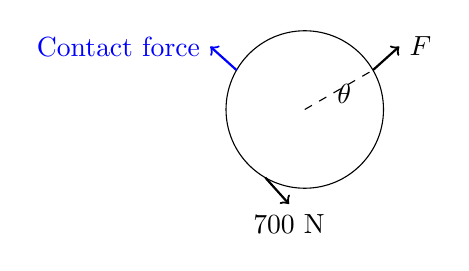
\begin{tikzpicture}
\draw (0,0) circle (1cm);
\draw[->,thick] (0.866,0.5) -- (1.2,0.8) node[right] {$F$};
\draw[->,thick] (-0.5,-0.866) -- (-0.2,-1.2) node[below] {$700\ \mathrm{N}$};
\draw[->,thick,blue] (-0.866,0.5) -- (-1.2,0.8) node[left] {Contact force};
\draw[dashed] (0,0) -- (0.866,0.5);
\draw (0.5,0.2) node {$\theta$};
\end{tikzpicture}
\end{center}
Contact force at $P$ acts along the radius toward the centre (since no friction at point of contact when just losing contact with ground? Actually at the instant, the wheel is in contact only at $P$, and the kerb exerts a force perpendicular to the surface (normal force) which points toward the centre of the wheel. So arrow from $P$ toward centre.
\end{frame}

\begin{frame}{NJC 2025 P2 Q3 – Solution (c)}
(c) Using principle of moments and taking moments about P:
$700 \times 0.60 \sin 30 = F(1.20 - 0.08)$
$F = 187.5 \approx 188\ \mathrm{N} = 190\ \mathrm{N}$.
\end{frame}

\begin{frame}{NJC 2025 P2 Q3 – Solution (d)}
Contact force at $P$ is the resultant of normal and friction. Using vertical equilibrium: $R_y = 700\ \mathrm{N}$. Horizontal equilibrium: $R_x = F = 190\ \mathrm{N}$. So magnitude $R = \sqrt{700^2 + 190^2} = \sqrt{490000 + 36100} = \sqrt{526100} \approx 725\ \mathrm{N}$.
\end{frame}

% HCI 2025 P2 Q2 (cantilever)
\begin{frame}[shrink=15]{HCI 2025 H2 Physics Prelim Paper 2 Q2}
A cantilever is set up on a rough table using a rigid uniform metre rule of mass $0.11\ \mathrm{kg}$, a $1.5\ \mathrm{kg}$ block and a $5.0\ \mathrm{g}$ mass as shown. Determine the maximum number of $5.0\ \mathrm{g}$ masses that can be stacked above point X such that the cantilever does not topple.
\end{frame}

\begin{frame}[shrink=15]{HCI 2025 P2 Q2 – Solution}
Let $n$ be number of $5.0\ \mathrm{g}$ masses. Take moments about the edge of the table (the pivot point). The metre rule extends $0.50\ \mathrm{m}$ over the edge? The diagram shows the rule has the block at the left end, and masses at X near the right end. We need details from the solution. From HCI P2 Ans.pdf page 2:
Anticlockwise moments: $(1.5g)(0.05)$? Actually they write: $(1.5g)(0.05) = (0.11g)(0.40) + n(0.005g)(0.80)$. Solving gives $n = 7$.
Thus maximum number is 7.
\end{frame}

% RI 2025 P2 Q2 (cantilever with modification)
\begin{frame}[shrink=15]{RI 2025 H2 Physics Prelim Paper 2 Q2}
A cantilever is set up using a rigid uniform metre rule of mass $0.11\ \mathrm{kg}$, a $1.5\ \mathrm{kg}$ block and a $5.0\ \mathrm{g}$ mass. (a) Determine the maximum number of $5.0\ \mathrm{g}$ masses that can be stacked above point X such that the cantilever does not topple. (b) The structure is modified by adding an inextensible string that passes over a frictionless pulley with its ends tied to the $1.5\ \mathrm{kg}$ block and to the centre of the metre rule. State and explain how this modification will affect your answer in (a).
\end{frame}

\begin{frame}{RI 2025 P2 Q2 – Solution (a)}
Similar to HCI Q2, the solution yields $n = 7$. (Check RI P2 Ans.pdf page 1: they get 7.)
\end{frame}

\begin{frame}[shrink=15]{RI 2025 P2 Q2 – Solution (b)}
Solution to be added.
\end{frame}

\subsection{Paper 3}

% Section 4: Question Bank
\section{Question Bank}

\subsection{Torque and Equilibrium (H2 Level)}

\begin{frame}[shrink=15]{Variation 1 – Seesaw Balance \hfill Difficulty: 2/10}
A $3.0\ \mathrm{m}$ long uniform plank of mass $20\ \mathrm{kg}$ is pivoted at its centre. A $30\ \mathrm{kg}$ child sits at one end. Where must a $40\ \mathrm{kg}$ child sit to balance?
\end{frame}

\begin{frame}{Variation 1 – Solution}
Let distance from pivot for $40\ \mathrm{kg}$ child be $d$. Taking moments about pivot:
$30g \times 1.5 = 40g \times d$ (plank's weight acts at pivot, no moment).
$d = (30\times1.5)/40 = 45/40 = 1.125\ \mathrm{m}$ from pivot on opposite side.
\end{frame}

\begin{frame}[shrink=15]{Variation 2 – Ladder Against Wall \hfill Difficulty: 5/10}
A uniform ladder of length $5.0\ \mathrm{m}$ and mass $15\ \mathrm{kg}$ rests against a smooth vertical wall and rough horizontal ground ($\mu = 0.40$). The ladder makes $60^\circ$ with the ground. How far up the ladder can a $70\ \mathrm{kg}$ person climb before the ladder slips?
\end{frame}

\begin{frame}[shrink=15]{Variation 2 – Solution}
Forces: weight of ladder $W_l$ at centre, person $W_p$ at distance $x$ from bottom, normal at wall $N_w$ horizontal, normal at ground $N_g$ vertical, friction $f = \mu N_g$ horizontal.
Vertical equilibrium: $N_g = W_l + W_p = (15+70)g = 85g$.
Horizontal: $f = N_w$.
Moments about bottom: $N_w \times 5\sin60^\circ = W_l \times 2.5\cos60^\circ + W_p \times x\cos60^\circ$.
$N_w = \mu N_g = 0.4\times85g = 34g$.
Left side: $34g \times 5\times0.8660 = 34g \times 4.33 = 147.22g$.
Right side: $15g \times 2.5\times0.5 + 70g \times x\times0.5 = 18.75g + 35g x$.
Thus $147.22g = 18.75g + 35g x \Rightarrow 128.47 = 35x \Rightarrow x \approx 3.67\ \mathrm{m}$ from bottom.
\end{frame}

\begin{frame}[shrink=15]{Variation 3 – Hinged Beam \hfill Difficulty: 4/10}
A uniform beam of mass $10\ \mathrm{kg}$ and length $4.0\ \mathrm{m}$ is hinged at one end and supported by a cable at the other end making $30^\circ$ with the beam. Find the tension in the cable.
\end{frame}

\begin{frame}{Variation 3 – Solution}
Forces: weight $W = 10g$ at centre, tension $T$ at end at $30^\circ$ to beam (so vertical component $T\sin30$, horizontal $T\cos30$). Hinge reaction $R$ at pivot. Take moments about hinge: $W \times 2\cos\theta_{\text{beam}}$? The beam is horizontal? Assume horizontal. Weight moment $= 10g \times 2$ (since weight at centre, distance 2 m). Tension moment: vertical component $T\sin30$ acts at end, distance $4$ m, so anticlockwise moment $= T\sin30 \times 4$. Horizontal component has zero moment about hinge. Equilibrium: $4T\sin30 = 20g \Rightarrow 4T\times0.5 = 20g \Rightarrow 2T = 20g \Rightarrow T = 10g = 98.1\ \mathrm{N}$.
\end{frame}

\begin{frame}[shrink=15]{Variation 4 – Shelf Brackets \hfill Difficulty: 3/10}
A shelf of weight $50\ \mathrm{N}$ and length $1.2\ \mathrm{m}$ is attached to a wall by a hinge at one end and a supporting wire at the other end at $45^\circ$ to the horizontal. Find the tension in the wire.
\end{frame}

\begin{frame}{Variation 4 – Solution}
Take moments about hinge: weight $50\ \mathrm{N}$ acts at centre ($0.6\ \mathrm{m}$ from hinge). Tension $T$ at end ($1.2\ \mathrm{m}$) has vertical component $T\sin45$. Moment: $T\sin45\times1.2 = 50\times0.6 = 30$. $T\times0.7071\times1.2 = 30 \Rightarrow 0.8485T = 30 \Rightarrow T \approx 35.4\ \mathrm{N}$.
\end{frame}

\subsection{Rotational Dynamics (H2 Level)}

\begin{frame}[shrink=15]{Variation 5 – Flywheel Acceleration \hfill Difficulty: 4/10}
A flywheel of moment of inertia $0.5\ \mathrm{kg\,m^2}$ is subjected to a constant torque of $2.0\ \mathrm{Nm}$. Starting from rest, find its angular velocity after $5.0\ \mathrm{s}$ and the number of revolutions turned.
\end{frame}

\begin{frame}{Variation 5 – Solution}
Angular acceleration $\alpha = \tau / I = 2.0 / 0.5 = 4.0\ \mathrm{rad/s^2}$.
After $5\ \mathrm{s}$: $\omega = \alpha t = 4\times5 = 20\ \mathrm{rad/s}$.
Angular displacement $\theta = \frac12 \alpha t^2 = 0.5\times4\times25 = 50\ \mathrm{rad}$.
Revolutions $= 50/(2\pi) \approx 7.96$.
\end{frame}

\begin{frame}[shrink=15]{Variation 6 – Atwood Machine with Massive Pulley \hfill Difficulty: 6/10}
Two masses $m_1 = 2\ \mathrm{kg}$ and $m_2 = 3\ \mathrm{kg}$ hang over a pulley of mass $1\ \mathrm{kg}$ and radius $0.1\ \mathrm{m}$ (disc, $I = \frac12 MR^2$). Find the acceleration of the masses.
\end{frame}

\begin{frame}[shrink=15]{Variation 6 – Solution}
Let $a$ be acceleration of masses. For $m_1$: $T_1 - m_1g = m_1 a$ upward? Actually set sign convention: let $m_2$ go down, $m_1$ up. For $m_2$: $m_2g - T_2 = m_2a$. For pulley: $(T_2 - T_1)R = I \alpha$, with $\alpha = a/R$. $I = \frac12 M R^2 = 0.5\times1\times0.01 = 0.005\ \mathrm{kg\,m^2}$. So $(T_2 - T_1)R = 0.005 \times a/R = 0.005 a / R$. Multiply by $R$: $T_2 - T_1 = 0.005 a / R^2 = 0.005 a / 0.01 = 0.5 a$.
Now solve: $T_1 = m_1(g + a)$, $T_2 = m_2(g - a)$. Substitute: $m_2(g - a) - m_1(g + a) = 0.5a$.
$3(9.81 - a) - 2(9.81 + a) = 0.5a \Rightarrow 29.43 - 3a - 19.62 - 2a = 0.5a \Rightarrow 9.81 - 5a = 0.5a \Rightarrow 9.81 = 5.5a \Rightarrow a \approx 1.78\ \mathrm{m/s^2}$.
\end{frame}

\begin{frame}[shrink=15]{Variation 7 – Rotating Rod \hfill Difficulty: 5/10}
A uniform rod of length $L = 1.0\ \mathrm{m}$ and mass $2\ \mathrm{kg}$ is pivoted at one end and released from horizontal. Find its angular velocity when it becomes vertical.
\end{frame}

\begin{frame}{Variation 7 – Solution}
Moment of inertia about end: $I = \frac13 ML^2 = \frac13 \times2\times1^2 = \frac23\ \mathrm{kg\,m^2}$.
Centre of mass falls a distance $L/2 = 0.5\ \mathrm{m}$. Energy conservation: $Mg\frac{L}{2} = \frac12 I \omega^2$.
$2\times9.81\times0.5 = 9.81 = \frac12 \times \frac23 \times \omega^2 = \frac13 \omega^2$.
$\omega^2 = 29.43$, $\omega \approx 5.43\ \mathrm{rad/s}$.
\end{frame}

\subsection{Angular Momentum (H2 Level)}

\begin{frame}[shrink=15]{Variation 8 – Skater Spins \hfill Difficulty: 3/10}
A skater spins at $2.0\ \mathrm{rev/s}$ with arms out, moment of inertia $3.0\ \mathrm{kg\,m^2}$. She pulls arms in, reducing $I$ to $1.2\ \mathrm{kg\,m^2}$. Find her new angular speed.
\end{frame}

\begin{frame}{Variation 8 – Solution}
Conservation of angular momentum: $I_1\omega_1 = I_2\omega_2$. $\omega_1 = 2\times2\pi = 4\pi\ \mathrm{rad/s}$.
$\omega_2 = I_1\omega_1/I_2 = 3\times4\pi/1.2 = 12\pi/1.2 = 10\pi\ \mathrm{rad/s} = 5\ \mathrm{rev/s}$.
\end{frame}

\begin{frame}[shrink=15]{Variation 9 – Collision with Pivot \hfill Difficulty: 5/10}
A door (width $1.0\ \mathrm{m}$, mass $15\ \mathrm{kg}$, hinged at one end) is at rest. A ball of mass $0.5\ \mathrm{kg}$ moving at $10\ \mathrm{m/s}$ strikes the door perpendicularly at its centre and sticks. Find the angular speed of the door after impact.
\end{frame}

\begin{frame}{Variation 9 – Solution}
Moment of inertia of door about hinges: $I_d = \frac13 M L^2 = \frac13 \times15\times1^2 = 5\ \mathrm{kg\,m^2}$.
Ball's angular momentum about hinges before impact: $L_{\text{ball}} = m v r = 0.5\times10\times0.5 = 2.5\ \mathrm{kg\,m^2/s}$.
After sticking, total $I = I_d + m r^2 = 5 + 0.5\times0.25 = 5.125\ \mathrm{kg\,m^2}$.
Angular momentum conserved: $2.5 = 5.125\,\omega \Rightarrow \omega \approx 0.488\ \mathrm{rad/s}$.
\end{frame}

\subsection{Rolling Motion (H2 Level)}

\begin{frame}[shrink=15]{Variation 10 – Rolling Down Incline \hfill Difficulty: 4/10}
A solid sphere (mass $2\ \mathrm{kg}$, radius $0.1\ \mathrm{m}$) rolls without slipping down a $30^\circ$ incline of length $2\ \mathrm{m}$. Find its speed at the bottom.
\end{frame}

\begin{frame}{Variation 10 – Solution}
Energy conservation: $mgh = \frac12 m v^2 + \frac12 I \omega^2$, with $I = \frac25 m R^2$, $\omega = v/R$.
$mgh = \frac12 m v^2 + \frac12 (\frac25 m R^2)(v^2/R^2) = \frac12 m v^2 (1 + \frac25) = \frac12 m v^2 \times \frac75$.
$gh = \frac{7}{10} v^2 \Rightarrow v = \sqrt{\frac{10}{7} g h}$.
$h = 2\sin30^\circ = 1\ \mathrm{m}$. $v = \sqrt{\frac{10}{7}\times9.81} \approx \sqrt{14.014} \approx 3.74\ \mathrm{m/s}$.
\end{frame}

\begin{frame}[shrink=15]{Variation 11 – Yo-yo \hfill Difficulty: 5/10}
A yo-yo of mass $0.1\ \mathrm{kg}$ and moment of inertia $I = 5\times10^{-5}\ \mathrm{kg\,m^2}$ has string wrapped around axle of radius $0.01\ \mathrm{m}$. It is released from rest. Find acceleration.
\end{frame}

\begin{frame}{Variation 11 – Solution}
Forces: $mg - T = ma$. Torque: $T r = I \alpha$, with $a = \alpha r$. So $T = I a / r^2$.
Substitute: $mg - I a / r^2 = ma \Rightarrow mg = a (m + I/r^2)$.
$a = \frac{mg}{m + I/r^2} = \frac{0.1\times9.81}{0.1 + 5\times10^{-5}/10^{-4}} = \frac{0.981}{0.1 + 0.5} = \frac{0.981}{0.6} \approx 1.635\ \mathrm{m/s^2}$.
\end{frame}

\subsection{Challenge Problems (H3 / Competition)}

\begin{frame}[shrink=15]{Challenge 1 – Pivoted Rod with Hanging Mass \hfill Difficulty: 7/10}
A uniform rod of mass $M$ and length $L$ is pivoted at one end. A mass $m$ is attached to the other end. The rod is released from horizontal. Find the angular speed when vertical.
\end{frame}

\begin{frame}{Challenge 1 – Solution}
Moment of inertia: $I = \frac13 ML^2 + m L^2$.
Centre of mass of rod at $L/2$, mass $m$ at $L$. Potential energy change: $\Delta U = Mg\frac{L}{2} + mgL = gL\left(\frac{M}{2} + m\right)$.
Energy: $\Delta U = \frac12 I \omega^2$.
$\omega^2 = \frac{2gL\left(\frac{M}{2}+m\right)}{\frac13 ML^2 + m L^2} = \frac{2g\left(\frac{M}{2}+m\right)}{L\left(\frac13 M + m\right)}$.
\end{frame}

\begin{frame}[shrink=15]{Challenge 2 – Rotating Collision \hfill Difficulty: 8/10}
A uniform rod of mass $M$ and length $L$ is pivoted at its centre. A particle of mass $m$ moving with speed $v$ strikes one end perpendicularly and sticks. Find angular speed of system after collision.
\end{frame}

\begin{frame}{Challenge 2 – Solution}
Before collision, angular momentum about pivot: $L_i = m v (L/2)$ (since particle strikes at end, distance $L/2$ from centre). After sticking, total moment of inertia: $I = \frac{1}{12} M L^2 + m (L/2)^2 = \frac{1}{12} M L^2 + \frac14 m L^2$.
Angular momentum conserved: $m v L/2 = I \omega$.
$\omega = \frac{m v L/2}{\frac{1}{12} M L^2 + \frac14 m L^2} = \frac{m v /2}{L\left(\frac{1}{12} M + \frac14 m\right)}$.
\end{frame}

\begin{frame}[shrink=15]{Challenge 3 – Rolling on a Loop \hfill Difficulty: 9/10}
A small solid sphere rolls without slipping from rest at height $h$ on a track that leads into a vertical loop of radius $R$. Find the minimum $h$ so that the sphere completes the loop without losing contact.
\end{frame}

\begin{frame}[shrink=15]{Challenge 3 – Solution}
At top of loop, speed must satisfy $mg + N = mv^2/R$, with $N \ge 0$ so $v^2 \ge gR$. For rolling sphere, $v = \omega R$, $I = \frac25 mR^2$.
Energy from start to top: $mg(h - 2R) = \frac12 m v^2 + \frac12 I \omega^2 = \frac12 m v^2 + \frac12 \cdot \frac25 mR^2 \cdot (v^2/R^2) = \frac12 m v^2 (1 + \frac25) = \frac{7}{10} m v^2$.
Thus $g(h - 2R) = \frac{7}{10} v^2 \ge \frac{7}{10} gR \Rightarrow h - 2R \ge \frac{7}{10} R \Rightarrow h \ge 2.7 R$.
\end{frame}

\begin{frame}[shrink=15]{Challenge 4 – Gyroscope Precession \hfill Difficulty: 9/10}
A gyroscope consists of a disc of mass $m$ and radius $r$ spinning at angular speed $\omega$ on an axle of length $L$ pivoted at one end. Find the precession angular speed $\Omega$.
\end{frame}

\begin{frame}{Challenge 4 – Solution}
Torque due to weight: $\tau = mgL$ (horizontal). Angular momentum of disc: $L_{\text{spin}} = I \omega = \frac12 m r^2 \omega$.
Precession rate $\Omega = \tau / L_{\text{spin}} = \frac{mgL}{\frac12 m r^2 \omega} = \frac{2gL}{r^2 \omega}$.
\end{frame}

\begin{frame}[shrink=15]{Challenge 5 – Falling Chimney \hfill Difficulty: 8/10}
A tall uniform chimney of height $H$ and mass $M$ is hinged at the bottom and falls over. Find the angular speed when it makes angle $\theta$ with the vertical, and determine the point where it might break (stress maximum).
\end{frame}

\begin{frame}[shrink=15]{Challenge 5 – Solution}
Moment of inertia about bottom: $I = \frac13 M H^2$. Centre of mass falls distance $\frac{H}{2}(1-\cos\theta)$. Energy: $Mg\frac{H}{2}(1-\cos\theta) = \frac12 I \omega^2 = \frac12 \cdot \frac13 M H^2 \omega^2 \Rightarrow \omega^2 = \frac{3g}{H}(1-\cos\theta)$.
The bending moment is maximum at a point about $1/3$ from bottom, which is where chimney often breaks.
\end{frame}

% Section 5: Synthesis & Consolidation
\section{Synthesis \& Consolidation}

\begin{frame}{End‑of‑Session Concept Recap}
\begin{itemize}
    \item Torque = force × perpendicular distance from pivot.
    \item Rotational equilibrium: sum of torques = 0.
    \item Moment of inertia $I$ depends on mass distribution.
    \item Rotational dynamics: $\tau_{\text{net}} = I\alpha$.
    \item Rotational kinetic energy: $K_{\text{rot}} = \frac12 I\omega^2$.
    \item Angular momentum $L = I\omega$, conserved if no external torque.
    \item Rolling without slipping: $v = \omega R$, total KE = translational + rotational.
    \item Applications: seesaws, ladders, flywheels, spinning skaters, rolling objects.
\end{itemize}
\end{frame}

\begin{frame}{Mind Map}
\centering
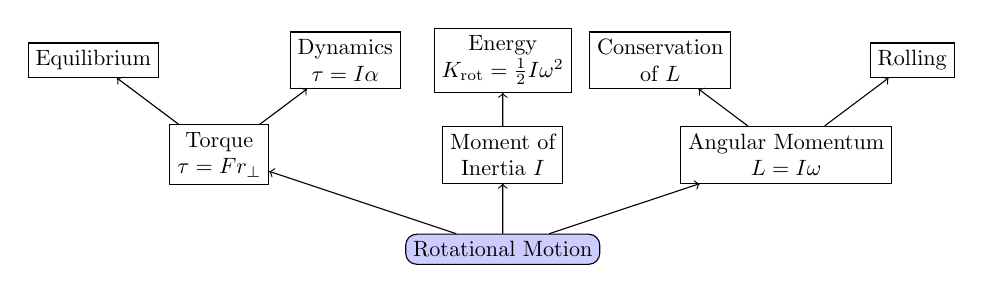
\begin{tikzpicture}[scale=0.8, transform shape]

% Root Node
\node[draw,rounded corners,fill=blue!20] (root) at (0,0) {Rotational Motion};

% Level 1: Categories
\node[draw, align=center] (torque) at (-4.5,1.5) {Torque \\ $\tau = Fr_\perp$};
\node[draw, align=center] (moi) at (0,1.5) {Moment of \\ Inertia $I$};
\node[draw, align=center] (angmom) at (4.5,1.5) {Angular Momentum \\ $L = I\omega$};

% Level 2: Sub-topics
% Children of Torque
\node[draw] (eq) at (-6.5,3) {Equilibrium};
\node[draw, align=center] (dyn) at (-2.5,3) {Dynamics \\ $\tau = I\alpha$};

% Child of Moment of Inertia
\node[draw, align=center] (energy) at (0,3) {Energy \\ $K_{\text{rot}} = \frac12 I\omega^2$};

% Children of Angular Momentum
\node[draw, align=center] (cons) at (2.5,3) {Conservation \\ of $L$};
\node[draw] (roll) at (6.5,3) {Rolling};

% Arrows (Root to Level 1)
\draw[->] (root) -- (torque);
\draw[->] (root) -- (moi);
\draw[->] (root) -- (angmom);

% Arrows (Level 1 to Level 2)
\draw[->] (torque) -- (eq);
\draw[->] (torque) -- (dyn);

\draw[->] (moi) -- (energy);

\draw[->] (angmom) -- (cons);
\draw[->] (angmom) -- (roll);

\end{tikzpicture}
\vfill
Link to linear motion: analogous quantities – force/torque, mass/moment of inertia, linear momentum/angular momentum.
\end{frame}

\end{document}
